	\documentclass[finnish,12pt]{article}
	\usepackage{aaltothesis}
	
      % \usepackage[T1]{inputenc}


	%% Use this if you run latex and use eps-format pictures
	%\usepackage[dvips]{graphicx}
	\usepackage[pdftex]{graphicx} 
	\usepackage{subfigure}

	\pdfoptionalwaysusepdfpagebox=5
	
	\makeindex
	\usepackage[pdfpagemode=None,colorlinks=false,urlcolor=red,linkcolor=blue,citecolor=black,pdfstartview=FitH]{hyperref}

	%% Use this if you do not like hyperref package - this defines url environment and formats it correctly
	%\usepackage{url}

	% Math stuff
	\usepackage{amsfonts,amssymb,amsbsy}

	\usepackage{setspace}
	\onehalfspacing
	\setlength\parindent{0pt}
	\usepackage[parfill]{parskip}
	
	\usepackage{lmodern}
	
	% Layout
	\setlength{\hoffset}{-1in}
	\setlength{\oddsidemargin}{35mm}
	\setlength{\evensidemargin}{25mm}
	\setlength{\textwidth}{15cm}
	\setlength{\voffset}{-1in}
	\setlength{\headsep}{7mm}
	\setlength{\headheight}{1em}
	\setlength{\topmargin}{25mm-\headheight-\headsep}
	\setlength{\textheight}{23cm}

	\bibliographystyle{unsrt}

	\uselogo{blue}{?}{tkk}
	\university{}{Aalto-yliopisto}
	\school{}{Sähkötekniikan korkeakoulu}
	\faculty{}{Automaatio- ja systeemitekniikan laitos}
	\degreeprogram{}{Automaatio- ja systeemitekniikka}
	\univdegree{BSc}
	\author{Ian Tuomi}{}
	\thesistitle{}{Teollisen ohjausjärjestelmän logiikkakuvauksen muuntaminen esteettiseksi kaavioksi}

	\place{Espoo}
	\date{6.12.2012}
	\supervisor{DI Mika Str\"{o}mman}{DI Marek Matusiak}
	\instructor{}{DI Mika Str\"{o}mman}

	\keywords{Automaatiojärjestelmä, Automatisoitu suunnittelu, ohjelmoitava logiikka, PLC, IEC 61131, FBD, graafinpiirto, suunnattu graafi}

	\begin{document}

	 \makecoverpage

	\begin{abstractpage}[finnish]
Työssä esitellään automaatiosuunnitteluun liittyviä malleja, kuvauksia ja metamalleja, sekä niiden esitystapoja jaetussa suunnittelutietokannassa.
Logiikan kaaviomuotoista esitystä esitellään.

Esteettisen kaavion tunnusmerkit määritellään, ja esitellään menetelmä, jonka tuloksena sellainen voidaan laatia.
Menetelmän vaiheet ja niihin liittyviä algoritmeja esitellään.
	\end{abstractpage}

	\newpage

	\mysection{Esipuhe}

On paljon ihmisiä, joita ilman tämä työ ei olisi toteutunut.
Haluan kiittää erityisesti seuraavia ihmisiä.

Työn ohjaajaa Mika Strömmania tarkoista huomioista ja rakentavista keskusteluista.

Petri Kokkoa ja Pekka Niemistä suunnannäytöstä ja ideoista.

Kandiryhmäni jäseniä
Peter 'Bembu' Kronströmiä,
Lauri Vepsäläistä,
Heikki 'Taffis' Tahvanaista,
Panu Kauppista
ja Lauri Andleria
vertaistuesta ja hyvästä yhteishengestä.

Aalto-yliopiston henkilökuntaa ja kurssin järjestäjiä hyvästä työstä.

Vanhempiani tuesta ja kannustuksesta.

	\vspace{5cm}

Otaniemessä itsenäisyyspäivänä 6.12.2012

\vspace{1mm}
	{\hfill Ian Tuomi \hspace{1cm}}

	\newpage

	\tableofcontents

\addcontentsline{toc}{section}{Sisällysluettelo}


%% Käsitteet
	\mysection{Lyhenteet}

	\begin{tabular}{ll}	     	    
DCS	& Distributed Control System \\
	& Hajautettu ohjausjärjestelmä \\ \\
DFS	& Depth-first search\\
	& Syvyyssuuntainen läpikäynti \\\\

FBD	& Function Block Diagram\\
	& IEC 61131-3 standardin määrittelemä ohjelmointikieli\\\\
IEC	& International Electrotechnical Commission,\\
	& Kansainvälinen sähköalan standarointiorganisaatio\\\\
NP & Nondeterministic Polynomial time\\
	& Epädeterministisellä Turingin koneella polynomiaalisessa\\&ajassa ratkeavien ongelmien joukko \\\\ 
PI	& Prosessien instrumentointi\\\\
PLC	& Programmable Logic Circuit \\
	& Ohjelmoitava logiikkapiiri\\\\
XML	& Extensible Markup Language\\
	& Merkintäkieli johon voidaan sisällyttää ja jolla voidaan jäsentää tietoa  \\\\
XSL	& Extensible Stylesheet Language\\
	& Kieliperhe, jolla voidaan määritellä ja muuntaa XML-formaatteja\\\\

\end{tabular}

	\cleardoublepage
	\storeinipagenumber
	\pagenumbering{arabic}
	\setcounter{page}{1}

% Kandi %

	\section{Johdanto}
	\thispagestyle{empty}

Teollista automaatiojärjestelmää suunnitteltaessa tuotetaan suuri määrä erilaisia dokumentteja.
Ne yhdessä muodostavat kuvauksen, joka mahdollistaa järjestelmän toteutuksen, käyttöönoton ja ylläpidon.
Dokumentaation laatiminen käsin on suurissa projekteissa työlästä ja tehotonta.
Nykyaikaisessa automaatio- ja instrumentointisuunnittelussa ongelma korostuu \cite{RefWorks:41}.
Ratkaisuista on tullut monimutkaisempia, ja laatu- ja joustavuusvaatimukset ovat lisääntyneet.
Lisäksi vaaditut toteutusajat ovat jatkuvasti lyhentyneet.

Johtuen suunnitteluprosessiin kohdistuneista vaatimuksista, työtä on pyritty tehostamaan automatisoiduilla apuvälineillä.
Metodiikka ei kuitenkaan ole ilmeisistä standardoimiseduista huolimatta yhtenäistynyt.
Automaatiosuunnittelun tutkimuskenttä on lisäksi hajanainen, ja yhteistyö on vähäistä.
Vaikka lähestymistavat ovat vaihtelevia, suunnittelussa on nähtävissä yhtenäinen siirtymä kohti jaettuja tietomalleja.
Automaatiojärjestelmien näkökulmasta jaettujen tietomallien käyttö tarkoittaa,
että suunnittelujärjestelmään tallentuu projektin edetessä kaikki sähköistys ja instrumentointi automaatiojärjestelmineen ja kenttälaitteineen.
Erilaiset kaaviot voidaan usein tuottaa suoraan tietomallin sisältävästä tietokannasta.

Tietomalliin perustuva lähestymistapa vaatii sen laajuuden ja rajoitukset määrittelevän metamallin.
Se ohjaa ja määrittää suunnittelun kohteen lisäksi myös yleisesti suunnittelutöiden kulkua.

Tämän kandidaatintyön kohteena on ohjausjärjestelmän logiikan muuntaminen standardeja noudattavaksi kaavioksi.
Logiikkakaavio on tapa pelkistää järjestelmän eri osien syöttöjen ja lähtöjen välillä vallitseva logiikka visuaaliseen ja helposti ymmärrettävään muotoon.
Se on määritelty yksiselitteisesti ja on tulkittavissa suunnatuksi graafiksi, jolloin algoritmillisen graafinpiirron tuloksia voidaan hyödyntää.

Algoritmillinen graafinasettelu on perusteellisesti tutkittu ala, jonka tuloksia voidaan käyttää kaikenlaisiin suunnattuihin graafeihin.
Tässä työssä eritellään Sugiyaman ym. \cite{RefWorks:9} esittämään hierarkiseen lähestymistapaan perustuva, logiikkakaavioiden kaltaisten tietovirtakaavioiden asetteluun soveltuva algoritmi.

Työssä on myös kokeellinen osio, jossa laadittua algoritmia käytetään konkreettisen kaavion asetteluun.
Lopuksi pohditaan tapoja sisällyttää menetelmä käytännön suunnittelutyöhön.

	\clearpage
	\section{Tehtaan mallit}

Tehdasmalli on kuvaus, joka mahdollistaa tehtaan toteutuksen, käyttöönoton ja ylläpidon.
Se on tietomalli, joka kuvaa tehtaan toimintaa, sen prosessia, organisaatiota, ihmisiä ja näitten aktiviteetteja.
Pohjimmiltaan se koostuu tehdasobjekteista ominaisuuksineen ja niitten välisistä relaatioista. \cite{RefWorks:41}

Suunnittelijoilla on työtehtävistään erilaisia tarpeita tehdasmallin suhteen.
Työn kohde on monitahoinen, eikä mikään yksi esitystapa pysty kattamaan kaikkia suunniteltavan järjestelmän näkymiä.
Tehdasta tulee kuvata useilta eri näkökannoilta erilaisilla tarkkuuksilla kunkin näkymän vaatimuksien mukaisesti.
Tehdasmalliin kuuluu siis useita malleja, jotka yhdessä muodostavat kokonaismallin.

Jokaisella mallilla on myös metamalli. Se määrittelee millaisia objekteja se voi sisältää, mitä ominaisuuksia sillä voi tai täytyy olla ja millaisia yhteyksiä objektien välillä on.
Metamallin loogiset riippuvuudet määrittelevät suunnittelun työtapoja ja järjestystä.
Ne kuvaavat millaiset tietomallit ovat suunnittelujärjestelmän kannalta hyväksyttäviä tehdasmalleja ja
määräävät sen laajuuden. Metamallin määritteleminen tekee työn tuloksesta ennakoitavan ja mahdollistaa tehokkaiden apuvälineiden kehittämisen.
Määrittelyllä myös suljetaan pois eriäviä tapoja kuvata tehdasta ja mahdollistetaan määrittelyyn perustuvat työkalut ja suunnittelukäytännöt.
Tällaisia ovat esimerkiksi uudelleenkäytettävää koodia sisältävät kirjastot ja erilaiset mallimuunnokset.

Suunnittelussa käytettävät metamallit valitaan siten, etteivät ne ole ristiriidassa ja muodostavat yhdessä toisiaan täydentävän kokonaisuuden.
Tällöin metamallien konfiguraatio muodostaa itsessään mallin.


	\subsection{Automaatiojärjestelmän kuvaukset}

Teollisuuden hajautettujen ohjausjärjestelmien suunnittelussa on havaittu
tarpeellisiksi ainakin kolme kuvausta: toiminnallinen, fyysinen sekä ohjelmistollinen \cite{RefWorks:38}.

		\subsubsection{Toiminnallinen kuvaus}

Toiminnallinen kuvaus määrittelee säätöjärjestelmän toiminnan tavalla, joka toteutettuna täyttää sille asetetut käyttäjävaatimukset.
Se kuvaa järjestelmän toimintaa, muttei määrää sen tarkkaa teknistä toteutusta. \cite{RefWorks:60}

Tätä näkymää määrittäessä voivat eri alojen suunnittelijat osallistua työhön ilman
tuntemusta instrumentoinnista tai ohjelmistokehityksestä. Kun päätökset on tehty
abstraktilla tasolla, voidaan hankinnat räätälöidä sen mukaisesti ja tulos
toteuttaa tehokkaasti.
Tällaisen määrittelyn avulla on mahdollista käyttää formaaleja verifiointimenetelmiä joitten avulla
voidaan osoittaa, että järjestelmän suunnitelma toteuttaa sille asetetut vaatimukset.
Näin suunnitelman oikeellisuus voidaan osoittaa ennen investointeja toteutukseen. \cite{RefWorks:41}

		\subsubsection{Fyysinen näkymä}

Fyysiseen näkymään suunnitellaan järjestelmän johdotukset, kaapelit, kenttäväylät,
ohjauskeskukset, toimilaitteiden sijainnit sekä ylipäänsä kaikki mitä vaaditaan 
järjestelmän fyysiseen käyttöönottoon. Sen käsittely ei kuulu tämän työn laajuteen.

		\subsubsection{Ohjelmistonäkymä}

Ohjelmistonäkymä kattaa funktionaalisen suunnittelun toteutuksen ohjelmamuodossa.
Asiakkaalla on yleensä omat toiveensa sen suhteen, millaiseen muotoon ohjelma tehdään.
Ohjelmiston toteuttamiseen ei pitäisi liittyä enää suunnittelutyötä - toisin sanoen toiminnallisen kuvauksen määrittelyjen täytyy olla riittävän tarkkoja jotta niitten mukaan tehdyssä ohjelmassa ei ole sen toimintaan vaikuttavia tulkinnanvaraisuuksia.

Ohjelmistototeutuksen työtavat jäävät usein määrittelemättömiksi ja muusta suunnittelutyöstä irrallisiksi,
vaikka pyrkimyksiä toteutustapojen nitten integroimiseksi suunnitteluprosessiin entistä vahvemmin on ollut.
Toteutustapa jää yksittäisten suunnittelijoiden määriteltäväksi, mistä seuraa että yhtenäistä työtapaa harvoin on.
Toteutetun ohjelmakoodin uudelleenkäyttö jää myös tyypillisesti vähäiselle asteelle. \cite{RefWorks:42}


	\subsection{Logiikan kuvaukset}

%McAvinew ym. \cite{RefWorks:53}
%Meier, automation body of knowledge: \cite{RefWorks:54}
%http://www.geocities.ws/andrikuncoro/Instrumentation/1811_06.pdf

Logiikan kuvaukset helpottavat tehtaan toiminnan ymmärrystä suunnittelu- ja rakennusvaiheen lisäksi tehtaan n ja huollon yhteydessä ja ovat siksi tärkeä osa tehtaan lopullista dokumentaatiota.
Teollisessa automaatiosuunnittelussa sallitut logiikan esitystavat on määritelty erityisesti selkeyttä, turvallisuutta ja ennustettavaa toimintaa silmälläpitäen.
Joskus loogista järjestelmää voidaan kuvailla kertomalla esimerkinomaisesti sen toiminnasta eri olosuhteissa.
Tällainen lähestymistapa ei kuitenkaan yleensä ole riittävä.
Lisäksi määritellään yleensä ainakin muuttujia, säätöpiirejä, sekvenssejä sekä niitten välisiä kytkentöjä.\cite{RefWorks:41}

Jatkuva prosessiohjaus voidaan esittää selkeästi järjestelmän PI-kaavioissa, mutta diskreetin ohjauksen esittämiseen tarvitaan erilaisia esityksiä, kuten logiikkadiagrammeja. \cite{RefWorks:54}

Logiikkadiagrammit kuvaavat syöttöjen ja lähtöjen välistä logiikkaa.
Määrittelyn mukaisia kaavioita ei kuitenkaan ole välttämättä helppoa laatia.

		\subsubsection{Toimintakaaviot}

Toimintakaavio on funktionaalisen näkymän toteutus, joka tavallisesti valmistellaan järjestelmän suunnittelun varhaisessa vaiheessa prosessikaaviosta.
Se määrittelee ohjausjärjestelmän toiminnot ja sitä pidetään ajantasaisena järjestelmän suunnittelun edetessä.
Se toimii suunnittelun apuna ja on lopulta osa lopullisen järjestelmän ohjeistusta.

Nykyaikaisessa automaation ohjelmistosuunnittelussa käytetään usein ohjelmointikieliä jotka ovat muodoltaan lähellä toiminnallisia logiikan kuvauksia ja dokumentoivat itsensä hyvin.
T'ämän vuoksi toiminnallinen kuvaus usein jätetään tekemättä, jolloin syntyy säästöjä. \cite{RefWorks:41}

		\subsubsection{Ohjelmakoodi}

Ohjelmakoodi on ohjelmanäkymän toteutus.
IEC~61131-3 on laajassa käytössä oleva avoin ohjelmakoodin standardi joka määrittelee automaatiologiikan ohjelmointimenetelmät ja pyrkii olemaan riittävän joustava mihin tahansa tarkoitukseen. \cite{RefWorks:62}
Se sisältää viisi erilaista ohjelmointikieltä, joista tässä työssä käsitellään erityisesti FBD:tä.

FBD-kieli koostuu toimilohkoista ja niiden välisistä langoista.
Toimilohkot kuvaavat toisistaan erillisiä itsenäisiä laskennallisia yksiköitä.
Langat kuvaavat niitten relaatioita toisiinsa.
Toimilohko voi tilastaan riippuen lähettää tapahtumia jotka vaikuttavat muitten toimilohkojen toimintaan.
Sen tekemien laskutoimitusten tulos riippuu sen vasemmalta puolelta tulevista syöttötiedoista ja sen suorittaman laskennan tulokset lähetetään blokin oikealta puolelta.
Toisiinsa liitetyt toimilohkot muodostavat verkon, joka määrittelee laajemman toiminnallisuuden. \cite{RefWorks:55}

Toimilohkojen muokkaamiseen on olemassa useita työkaluja.
Näistä mainitsemisen arvoisia ovat ainakin FBDK, 4DIAC ISaGRAF ja NxtControl.
Ne eivät kuitenkaan tarjoa kaavioiden asetteluun kuin yksinkertaisia työkaluja, jos ollenkaan.

Automaatiokaavioiden suoritusjärjestys etenee standardin IEC 61131-3 mukaan vasemmalta oikealle.
Lisäksi toimilohkoa ei ajeta ennen kuin kaikki sitä edeltävät toimilohkot on suoritettu.
Keskinäisen suoritusjärjestyksen täytyy myös tulla esille toteuttavassa ohjelmistossa.
Suoritusjärjestys kulkee usein ylhäältä alas, mutta tätä ei voi olettaa aina todeksi. \cite{RefWorks:62}

Suoritusjärjestysvaatimus asettaa seuraavassa kappaleessa tarkasteltavalle graafinpiirrolle rajoituksia.
Jos niitä ei oteta huomioon, saattaa graafin algoritmillinen piirto johtaa vääränlaiseen kaavioon.
Mahdollisten takaisinkytkentöjen tapauksessa vaaditaan huolellisuutta, jottei syklien poistovaiheessa kaavion järjestys muutu.


		\subsubsection{Logiikan tietokantakuvaukset}

Logiikka tallennetaan jaettuun suunnittelumalliin, johon kaikilla järjestelmän suunnittelijoilla on yhteys.
Tapa jolla logiikka tallennetaan täytyy olla yhdenmukainen, jotta suunnittelutyössä voidaan tehdä tehokasta yhteistyötä työpaikalla jaettujen yhtenäisten suunnittelun apuvälineiden avulla.
Lisäksi kuvauksen tulee olla formaali jotta logiikkaa voitaisiin käsitellä algoritmillisesti.
Formaalilla tarkoitetaan tietynlaista, tarkkaan määritetyn syntaksin mukaista kuvausta.
Tällöin tulee myös mahdolliseksi toteuttaa helposti tietoa käsitteleviä muunnosalgoritmeja.
Muunnoksella tarkoitetaan jonkin tiedon kuvauksen muuttamista toiseksi kuvaukseksi.

Standardin IEC 61131-3 mukaisten ohjelmointikielten kuvaamiseen on ehdotettu PLCopen-standardia.
Sen mukainen logiikan XML-muotoinen kuvaus voi sisältää toimilohkon toiminnallisuuden kannalta välttämättömien tietojen lisäksi toimilohkon sijainnin, koon ja jopa lankojen reititykset.
Esitys voidaan tällöin laatia siten, että se on tuotettavan kaavion asettelun kannalta täysin yksiselitteinen.
Tällaista kuvausta voidaan silloin pitää dokumentaation lopullisena muotona. \cite{RefWorks:64}

Kun logiikkakuvauksen muoto on määritelty tarkasti, voidaan määritelmän mukaisesti laadittu logiikkakuvaus muuntaa määritelmään nojaavien sääntöjen perusteella.
Monet automaatiologiikan suunnitteluohjelmistot pystyvät muuntamaan käyttämänsä kuvauksen PLCopen-muotoiseksi tiedoksi, jolloin suunnittelutietoa voidaan siirtää eri järjestelmien kesken.
Erilaisia XML-kuvauksia on helppoa laatia ja niitten sisältämien tietojen pohjalta voidaan tuottaa minkä tahansa muotoisia dokumentteja käyttäen hyväksi XSL-muunnoksia \cite{RefWorks:61}. Eri XML-pohjaisia tiedostoformaatteja käyttävien suunnitteluvälineiden välinen integraatio on tällöin helposti toteutettavissa.

Olemassaolevien suunnitteluohjelmistojen varaan rakennettu suunnittelujärjestelmä voi kuitenkin kohdata haasteita, jos luotetaan liikaa ohjelmien standardinmukaisuuteen.
Valmistajat jättävät usein standardinmukaisiksi kutsutuista ohjelmistoista määrittelyn mukaisia ominaisuuksia toteuttamatta.
Tämä siitä, että ohjelma on määritelty standardinmukaiseksi, jos se toteuttaa siitä jonkin osan ja mainitsee mitä se jättää toteuttamatta. \cite{RefWorks:42}


	\clearpage
		
	\section{Graafit ja niiden asettelu}

	\subsection{Määritelmiä}

Lähdetään liikkeelle graafin määritelmästä \cite{RefWorks:39}.
Graafi tai verkko on yleisen määritelmänsä mukaan joukko solmuja ja niitä yhteen liittäviä lankoja.
Lankoja kutsutaan usein myös kaariksi, reunoiksi, väleiksi tai linkeiksi. Solmusta käytetään myös ilmaisua noodi.
Matemaattisesti esitettynä graafi on joukko $G = (V, E)$, missä V on rajoitettu solmujoukko ja E on rajoitettu lankajoukko.

Kerrostus on jaottelu $\mathfrak{L} = (L_1, L_2, \dots, L_h)$, jonka alajoukot sisältävät yhdessä kaikki solmut $V$.
Solmujoukon erilaisia kerrostuksia vertaillaan jaottelun \emph{leveyden} ja \emph{korkeuden} avulla.
Korkeus\footnote{Tietovirtakaavioissa vasemmalta oikealle} on kerrosten määrä $h$ ja leveys\footnote{Tietovirtakaavioissa ylhäältä alas} on suurimman kerrosjoukon $L_i$ koko.

Laajennetaan määritelmää ja sisällytetään graafin määritelmään joukko portteja $P$ ja funktio $\mathsf{n} : P \rightarrow V$, joka kartoittaa portit niitä vastaaville solmuille.
Lanka koostuu porttiparista, joita se yhdistää. Graafi on \emph{suunnattu} silloin, kun sen langat ovat järjestettyjä pareja, joista toinen on tulo- ja toinen lähtöpiste. Toisinsanoen, $e = (p_1, p_2)$, missä $p_1$ on lähtö- ja $p_2$ tuloportti.

Solmu $v_j$ on solmun $v_i$ \emph{seuraaja} silloin, kun on olemassa lanka $e \in E$, jolle $\mathsf{n}(p_1) = v_i$ ja $\mathsf{n}(p_2) = v_j$.
Polku on solmusekvenssi $(v_1, v_2, \dots , v_k)$ jolle pätee, että $k>1$ ja jokainen sekvenssin solmu $v_{i+1}$ on solmun $v_i$ seuraaja.

Graafi on \emph{syklitön} silloin, kun mikään polku ei sisällä samaa solmua enemmän kuin kerran.
Lanka $(p_1, p_2)$ on \emph{itseohjautuva} silloin, kun $\mathsf{n}(p_1) = \mathsf{n}(p_2)$.
Kerrostus on \emph{kunnollinen}\footnote{eng. proper} silloin, kun jokaisen kerrostusjoukon $L_i$ jokaisen solmun seuraajat kuuluuvat kerrokseen $L_{i+1}$.

\emph{Virityspuu} on verkon aliverkko $G_s$ joka sisältää verkon kaikki solmut siten, että se sisältää mahdollisimman vähän lankoja.
Virityspuussa ei ole syklejä, koska mikä tahansa virityspuuksi ehdotetussa verkossa sijaitseva sykli $v_i, ... , v_i$ voidaan rikkoa poistamalla mikä tahansa yksittäinen sen sisältämistä langoista ilman, että sen sisältämän solmujoukon $E$ koko muuttuu.
Kun virityspuusta poistetaan lanka, jakaantuu puu kahdeksi.

 		\subsection{Tulosten arviointiperusteet}

Asetteluista halutaan mahdollisimman esteettisiä.
Estetiikka erittelee ominaisuudet mitä graafiin halutaan mahdollisimman paljon, jota se olisi mahdollismman luettava.
Asettelulle voidaan muodostaa 

Purchase ym. ovat tutkineet estetiikkaan vaikuttavia tekijöitä, ja he ovat määritelleet asettelun luettavuudelle tärkeimmikse seuraavat ominaisuudet: \cite{RefWorks:47} 
\begin{enumerate}
  \item Lankojen risteysmäärä
  \item Kaavion koko
  \item Lankojen yhteispituus
  \item Pisin lankapituus
  \item Symmetria
\end{enumerate}

Näistä ominaisuuksista lankojen risteysmäärä muodostui tärkeimmäksi. Myös lankojen pituus oli merkittävässä asemassa luettavuuden kannalta.
Esteettiset ominaisuudet ovat usein ristiriidassa keskenään.
Jotta voitaisiin esimerkiksi välttää langan piirto solmun läpi, joudutaan siihen usein tekemään mutkia.
Valmiin kaavion asettelua voidaan arvioida automatisoidusti laskemalla kaavioista esteettisyyteen vaikuttavia tekijöitä, kuten lankojen risteysmääriä.


	\subsection{Liittyvä työ}

Suunnattuja graafeja käytetään laajalti riippuvuussuhteiden mallintamiseen.
Esimerkkejä suunnatuista graafeista ovat projektinhallintaverkot, ontologioiden määrittelykaaviot, ohjelmien kutsupuut, syy-seurausdiagrammit sekä aiemmin osioissa 2.2.1 ja 2.2.2 käsittelemämme toimintakaaviot ja FBD-kieliset kaaviot.

Suurin osa graafinpiirrollisista lähestymistavoista on suunniteltu ennalta tuntemattomien verkkojen piirtämiseen.
Ne pyrkivät tuottamaan keskimäärin hyvän asettelun, oli graafi millainen hyvänsä.
Suunnatun verkon rakenteen huomioonottavat algoritmit tuottavat parempia tuloksia.
Tällaisia ovat kerrostetut asetteluemenetelmät.

Kerroksittainen tapa esittää syklittömiä ja suunnattuja verkkoja on intuitiivinen ja helppolukuinen.
Alkuperäinen ajatus graafien kerrostamisesta voidaan johtaa Warfieldin \cite{RefWorks:58} ja Carpanon \cite{RefWorks:57} esittämiin ajatuksiin graafiaasettelusta.
Ylivoimaisesti suosituin tapa suunnattujen graafien piirtoon on tällä Sugiyaman menetelmä. \cite{RefWorks:9}
Sugiyaman algoritmia ei voi kuitenkaan käyttää sellaisenaan tietovirtakaavioiden asetteluun.
Sitä onkin kehitetty valtavasti eteenpäin ja siihen on tehty sopivia laajennuksia riippuen käyttötarkoituksesta.
Tätä helpottaa menetemöän tkeähestymistapa jaottelee algoritmin vaiheisiin, joista jokaista voidaan tutkia erillisenä ongelmana.
Sen määrittelemä jaottelu on säilynyt hierarkisen graafinpiirron tutkimuskentässä ajankohtaisena, vaikkei sen esittämiä algoritmeja käytetäkään.

Aseteltavissa tietovirtakaavioissa esiintyvät toimilohkot sisältävät useita portteja, joiden keskinäinen järjestys on säilytettävä.
Lisäksi langat ovat tietovirtakaavioissa yleisen käytännön mukaisesti ortogonaalisia, jolloin algoritmia pitää täydentää erillisellä langoille tarkoitetulla reititysalgortimilla.

Työvaiheista kerrostus ja risteyksien vähennysvaihe saattavat muuttaa suoritusjärjestystä.
Tällöin algoritmin toimintaa pitää yksinkertaisesti rajoittaa järjestysherkkien blokkien osalta.
Koska algoritmit ovat heuristisia, ovat siihen tehtävät yksinkertaiset rajoitukset helppoja toteuttaa.

Toimilohkojen syötöt ovat yleensä lohkon vasemmalla ja ulostulot oikealla puolella.
Näin on FBD-ohjelmointikielen tapauksessa aina.
Toimintakaavioiden tapauksessa syöttöjen ja ulostulojen sijainteja ei ole määritelty yhtä tarkasti, jolloin sivuportit on otettava asettelevassa algoritmissa myös huomioon jos sitä halutaan käyttää.
Sivuporttien huomioonottoon on esitetty ratkaisu, jossa lankojen reititystä varten asetetaan valesolmuja. \cite{RefWorks:51}

Laajoja käytännön tutkimuksia datavirtakaavioiden asettelusta on tehnyt Klauske ym.\cite{RefWorks:50}.
% TÄHÄN MYÖS JOKU MUU TAI OLET YHTÄ VAKUUTTAVA KUIN KASA PASKAA
\newpage

\begin{figure}[!p]
\centering
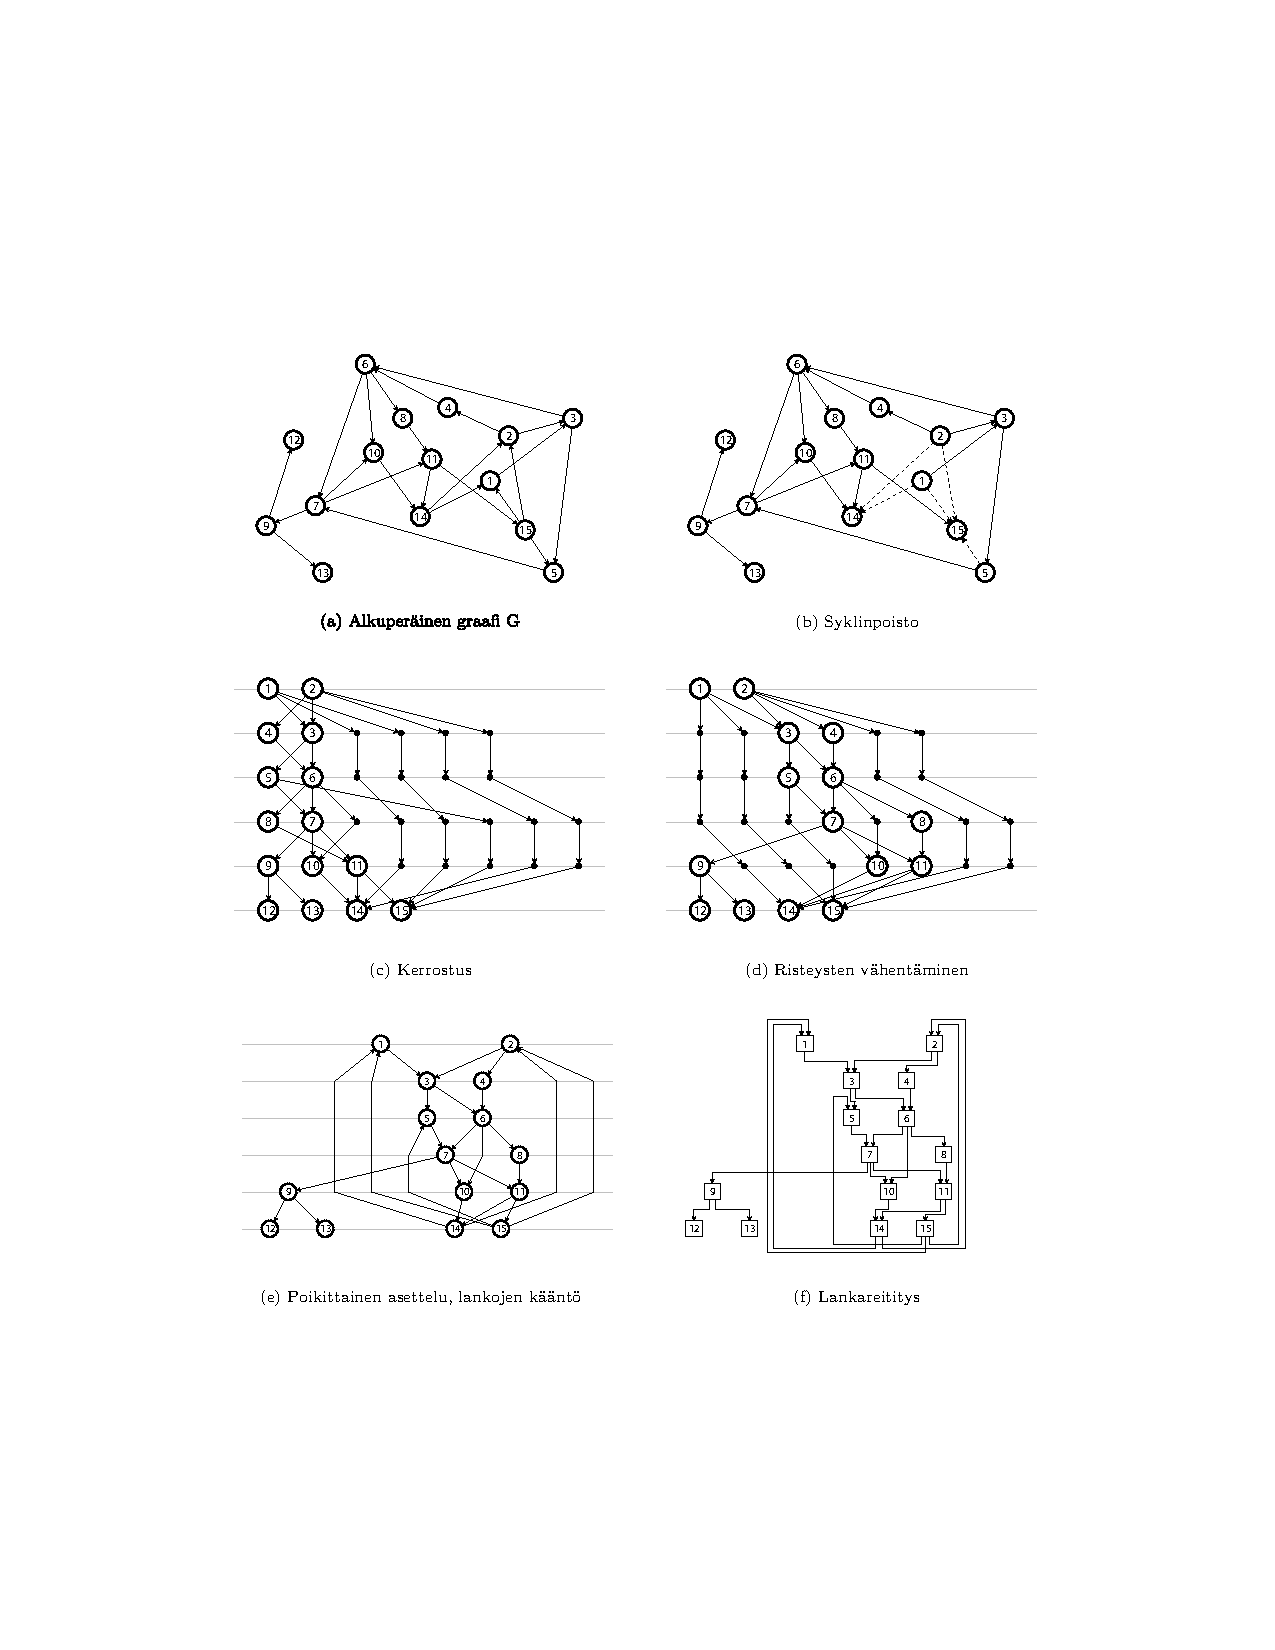
\includegraphics[width=\textwidth]{hier.pdf}
\caption{Sugiyaman menetelmän eri vaiheet (Healy ja Nikolov \cite{RefWorks:70}, lankareititys lisätty) . }
\end{figure}

		\subsection{Asettelualgoritmi}

Sugiyaman menetelmään perustuva asettelu koostuu viidestä eri vaiheesta, jotka on esitetty myös kuvassa 1.
\begin{enumerate}
  \item Syklien poisto, seuraa DFS-hakua \cite{RefWorks:69} tai Eades ym. ahnetta algoritmia \cite{RefWorks:48}
  \item Kerrostus, seuraa Gansner ym. lankapituuden minimimoivaa menetelmää. \cite{RefWorks:28}
  \item Risteysten vähentäminen, seuraa Sugiyama ym. alkuperäistä menetelmää. \cite{RefWorks:9}
  \item Poikittaisasettelu, seuraa Sanderin lineaaristen segmenttien menetelmää. \cite{RefWorks:49}
  \item Lankareititys, seuraa Sanderin monilankareititysalgoritmia. \cite{RefWorks:17}

\end{enumerate}

Algoritmin eri vaiheiden algoritmit on valittu ottaen huomioon datavirtauskaavioiden rajoitukset ja erityiset tarpeet sekä niitten rakenteelliset ominaisuudet.
Nämä vaiheet ovat toisistaan erillisiä ja voidaan tilanteen mukaan vaihtaa toisiksi tai jättää suorittamatta.
Jos esimerkiksi toimilohkojen paikat halutaan pitää paikallaan mutta laatia lankojen reititykset automaattisesti, voitaisiin päättää ajaa pelkästään algoritmin viides osio.
Seuraavaksi esitellään jokaisen vaiheen tavoitteet, niihin liittyvää tutkimustyötä sekä esitellään algoritmit työhön sovellettavilta osin.


		\subsubsection{Syklien poisto}

Syklinpoistovaiheessa muotoillaan graafi siten, että se on syklitön.
Syklit eli takaisinkytkennät ovat graafinpiirtoalgoritmien vaatimuksista huolimatta välttämätön osa kaavioita, eikä niitä voida kokonaan poistaa.
Tämän vuoksi syklit rikotaan kääntämällä yksi tai useampi syklin sisältämistä langoista.

Tarkemmin määriteltynä, tavoite on löytää mahdollisimman pieni lankajoukko $FS \subset E $ jonka sisältämät langat kääntämällä verkko on syklitön.
Tämä ongelman on osoitettu olevan NP-vaikea \cite{RefWorks:65}. 

Syklien poistovaiheessa käsiteltävä tietomalli sisältää tiedon jokaisessa puussa ensimmäisenä suoritettavista solmuista.
Tämä mahdollistaa huomattavan yksinkertaisten algoritmien käytön.
Yksi tällaisista menetelmistä mahdollisimman pienen lankajoukon $FS$ etsimiseen on DFS-haku.
DFS-haussa edetään ensimmäisenä suoritettavista solmuista mielivaltaista polkua pitkin, kääntäen matkalla kohdatut käänteiset langat. Tätä jatketaan kunnes luotua polkua $(e_1,e_2, ..., e_h)$ ei voida enää jatkaa.
Tämän jälkeen palataan polkua palataan taaksepäin lankaa $e_h$ pitkin ja yritetään edetä takaisin kunnes löydetään solmu josta lähtee lanka jota ei olla vielä seurattu. \cite{RefWorks:69}

Käännetyt langat käännetään lankojen reitittämisvaiheessa takaisin oikein päin käyttäen hyväksi lankajoukkoa $FS$.

Jos ensimmäinen kerros ei ole valmiiksi tiedossa tai sillä ei ole merkitystä, voidaan käyttää Berger-Shor algoritmiin \cite{RefWorks:68} perustuvaa ahnetta algoritmia \cite{RefWorks:48}.


		\subsubsection{Kerrostus}

Kerrostukselta vaaditaan, että se on kunnollinen sekä tiivis\footnote{eng. compact}.
Tiiviydellä tarkoitetaan, että kerrostuksen leveys ja pituus ovat pieniä ja kerrosten välinen etäisyys on vakio. 

Tämän saavuttamiseksi graafiin lisätään valesolmuja pitkien lankojen katkaisemiseksi.
Valesolmut ovat graafiin lisättäviä kuvitteellisia solmuja joita ei piirretä lopulliseen kaavioon, mutta jotka helpottavat sen algoritmillista käsittelyä.
Kerrostukseen halutaan valesolmuja mahdollisimman vähän tiiviyden, lyhyiden lankapituuksien sekä asettelun hyvän laskennallisen suoritusajan varmistamiseksi.

Tiiviyden äärimmäisenä rajoituksena toimii lopullisesta tarkastelutavasta riippuen näyttöpääte tai paperi, jolta aseteltua kaaviota on tarkoitus tarkastella.

Erilaisilla kerrostusmenetelmillä graafin pituus voidaan minimoida leveyden kustannuksella tai siitä voidaan tehdä mahdollisimman kapea pituuden kustannuksella.
Sekä leveyden että pituuden minimointi samanaikaisesti on rinnastettavissa multiprosessoriajastusongelmaan ja on siten NP-täydellinen ongelma. \cite{RefWorks:39}

Yksinkertainen tapa tuottaa kerrostus on pisimmän reitin tapa. Se asettaa ensin kaikki solmut, joilla ei ole seuraajia kerrokseen $L_1$.
Tämän jälkeen jokainen muu solmu asetetaan kerrokseen $L_{p+1}$, missä $p$ on lyhin etäisyys johonkin kerroksen $L_1$ solmuista.
Tällä tavalla laaditut kerrostukset sisältävät mahdollisimman vähän kerroksia.
Tämä lähestymistapa tuottaa kerrostukseen huomattavan suuria kerroksia.

Kun halutaan mahdollisimman kapeita kerrostuksia, on suotavaa käyttää multiprosessoriajastusongelman ratkaisemiseen kehitettyä Coffmann-Graham -algoritmia. \cite{RefWorks:59}
Ongelmana on ajastaa eri tehtävät $W$ kappaleelle prosessoreita siten, että kaikki tehtävät suoritetaan ajassa $H$.
Löydämme vastaavuuden verkon kerroksien määrälle ja suoritusajalle, sekä suurimmalle sallitulle kerroskoolle ja prosessorien määrälle.

Nämä kerrostusmenetelmät voivat olla hyödyllisiä sellaisissa sovelluksissa, joissa aseteltavan kaavion muodolla on erityisiä kapeus- tai pituusvaatimuksia.
Näitä ei sovelluksessamme ole, vaan tavoitteena on yksinkertaisesti mahdollisimman tiivis asettelu.
Huomataan, että kunnollisen kerrostuksen valesolmujen määrä on suoraan verrannollinen sen tiiviyteen.
On olemassa myös tapa laatia kerrostus, joka minimoi valesolmujen määrän ja voidaan vieläpä suorittaa polynomisessa ajassa.
Se löydetään kun otetaan käyttöön lineaarisen ohjelmoinnin optimointimenetelmä jolla minimoidaan

$$f=\displaystyle\sum\limits_{(v_1 ,v_2) \in V} (i - j - 1), \hspace{1.5cm} v_1 \in L_i \quad ja \quad v_2 \in L_j$$

Minimoitava arvo $f$ on samalla valesolmujen määrä.

Tälle lineaarisen ohjelmoinnin optimointiongelmalle on tehokas ratkaisutapa joka perustuu nk. \emph{Network Simplex}- algoritmiin\cite{RefWorks:28}. Sen aikakompleksisuutta ei ole pystytty osoittamaan, mutta se on käytännössä osoittautunut suoritusajaltaan erittäin nopeaksi, minkä seurauksena se on valittu tässä työssä käytettäväksi algoritmiksi.

Menetelmässä muodostetaan ensin verkon virityspuu.
Kun virityspuusta poistetaan jokin lanka, tuloksena syntyy kaksi toisistaan erillistä puuta, joista molemmat sisältävät eri solmut joita katkaistu lanka yhdisti.
Toinen sisältää langan lähde- ja toinen määränpääsolmun.
Näitten kahden puun perusteella lasketaan jokaiselle langalle \emph{leikkausarvo}.
Leikkausarvo on määränpääsolmun sisältävästä puusta ja lähdesolmun sisältävään puuhun kulkevien lankojen pituudet
josta vähennetään päinvastaiseen suuntaan kulkevien lankojen pituudet.

Negatiivinen leikkausarvo viittaa siihen, että kyseistä lankaa kannattaa todennäköisesti pidentää mahdollisimman paljon.
Tuloksena saadusta kerrostuksesta muodostetaan uusi virityspuu, ja menetelmää jatketaan edelleen kunnes kaikki virityspuun leikkausarvoista ovat positiivisia.


		\subsubsection{Risteyksien vähentäminen}

Lankojen risteysten määrä on osoittautunut olemaan suurin yksittäinen tekijä graafin luettavuuden kannalta. \cite{RefWorks:47}
Risteysmäärän vähentäminen pieneksi on tällöin mille tahansa luettavuutteen tähtäävälle asettelualgoritmille tärkeä tavoite.

Graafin kokonaisristeysmäärän vähentäminen ei perustu solmujen tarkkoihin sijainteihin, vaan niitten keskinäiseen järjestykseen.
Kahden kerroksen ylitysongelmassa etsitään joukolle $L_i$ järjestys, joka minimoi risteysten määrän kun joukko $L_{i+1}$ pysyy paikallaan.
Ongelma on siis luonteeltaan kombinatorinen eikä geometrinen, mikä huomattavasti yksinkertaistaa hyvän ratkaisun löytämistä.
Graafi on myös muokattu kerrostamisvaiheessa kelvolliseksi, minkä seurauksena ongelmaa ratkaistessa voidaan keskittyä vuorotellen vain kerrosparin $L_i$ ja $L_{i+1}$ välisiin lankoihin.
Näistä helpotuksista huolimatta kyseessä on NP-täydellinen ongelma siinäkin tapauksessa, että koko graafissa on kerroksia vain kaksi \cite{RefWorks:40}.

Parhaan mahdollisen kombinaation löytämiseksi joudutaan yksinkertaisen ratkaisun puutteessa käyttämään heuristisia menetelmiä.
Eräs suosittu lähestymistapa perustuu solmun seuraajasolmujen sijoittaminen sen kohdesolmujen mediaanin perusteella.
Teorian kannalta mediaanimenetelmällä on useita hyviä ominaisuuksia.
Sen avulla tuotetun ratkaisun risteysmäärän suhde parhaaseen mahdolliseen on vakio.
Lisäksi algoritmi voidaan suorittaa polynomisessa ajassa.
Käytännön kokeiluissa satunnaisilla graafeilla on kuitenkin todettu, ettei mediaaneihin perustuva menetelmä ole käyttökelpoisin. \cite{RefWorks:52}
Battisti ym. suosittelevatkin eri menetelmiä yhdisteleviä hybridialgoritmeja, kuten mediaanimenetelmän ja satunnaisten tranpositioiden yhdistämistä\cite{RefWorks:39}.

		\subsubsection{Poikittainen asettelu}

Jokainen kulma langassa aiheuttaa ylimääräisen rasitteen ihmisen hahmotuskyvylle. \cite{RefWorks:47}
Esteettistä lopputulosta tavoittelevan asettelualgoritmin tulee siis pyrkiä minimoimaan lankojen kulmat.
Siinä missä noodikerroksien noodikombinaatiot vaikuttavat lankojen risteysten määrään, vaikuttaa niiden tarkka poikittainen asettelu langoissa olevien kulmien määrään.
Solmujen poikittaisen asettelun avulla solmujen välisten lankojen käännösten määrää pyritään vähentämään jotta kaavion luettavuus paranee.
Asettelun merkitys korostuu kun lankoja on paljon, kuten automaation logiikkakaavioille on tyypillistä.

Risteysten vähentämisvaiheessa saavutettu kombinatorinen ratkaisu pyritään säilyttämään poikittaisasetteluvaiheessa.

Sander ehdottaa kaksivaiheista lähestymistapaa, jossa aluksi määritellään hyvä alkusijoittelu joka sitten tasapainoitetaan.
Solmujen suhteelliset sijainnit on jo määritelty aiemmissa vaiheissa.
Alkuperäisasettelussa solmut yksinkertaisesti jaetaan triviaalisti järjestyksessä .

Kun on saavutettu triviaali asettelu, voidaan siirtyä tasapainottamaan sitä.
Solmuasettelu tasapainoitetaan mallintamalla solmuja levossa olevina heilureina.
Solmut ovat heilurin päässä oleva paino ja lanka painoa kannatteleva naru.
Tasapainotettavaa kerrosta seuraava kerros pysyy kiinteänä paikoillaan.

Solmujen poikkeamat lasketaan ja vierekkäisten solmujen päällekkäisyyksien tapauksessa siirretään niitten muodostamia osioita kauemmaksi toisistaan kunnes päällekkäisyyksiä ei enää esiinny.

$$
D_p(e)=x(v_1)-x(v_2) \hspace{2cm} D_p(v)=\frac{\sum_{e \in E}D_p(e)}{indeg(v)}
$$

Segmentin siirtymä on sen sisältämien solmujen siirtymien summa, ja segmenttijoukon siirtymä on sen kaikkien segmenttien siirtymien keskiarvo

$$
D_p(S)=\sum_{v \in L} D_p(v)\hspace{2cm} D_p(v)=\frac{\sum_{i \in {1,...,k}}D_p(S_i)}{k}
$$


Kun solmujen sijainnit on tasapainotettu, jaotellaan asetteluun käytössä oleva tila ruudukoksi ja asetetaan solmut niitten tasapainotettuja sijainteja lähinnä oleviin ruudukkopisteisiin.
Menettely tekee kaaviosta vähemmän tasapainoisen, mutta käytännössä ruduukointi tekee siitä luettavamman.

		\subsubsection{Lankojen reititys}

Tietovirtakaavioiden toimilohkoissa on useita portteja ja niitten sisältämät lankareititykset ovat ortogonaalisia.
Nämä rajoitukset tulee ottaa tässä kaaviopiirron viimeisessä vaiheessa.
Gansner ym. esittivät porttiongelmaan ratkaisun, joka perustuu noodisijoitteluesityksen laajentamiseen porttien suhteellista sijaintia kuvaavalla tiedolla.\cite{RefWorks:28}

Kun jokaiselle solmulle on tiedossa niiden lopullinen sijainti, luodaan lankasegmenttejä siten, että ne liikkuvat solmujen koordinaattien välillä.
Poikittaiset segmentit jotka asetetaan tyhjään tilaan rivien $j$ ja $j+1$ välille saavat koordinaatikseen $j+0.5$.
Tämä toistetaan pystysuuntaisille segmenteille.

Kaikki samassa ruudussa tai sarakkeessa $k$ olevat segmentit kootaan ryhmäksi joukkoon $S$.
Tavoitteena on levittää ne koordinaateille välillä $[k, k+1]$.
Sander ym. ovat esittäneet reititysongelman ratkaisun, jossa käsitellään yksitellen jokaisen ruudun ylittävien lankasegmenttien muodostaman ryhmän paikallista asettelua erillisenä graafina. \cite{RefWorks:17}
Menetelmässä luodaan jokaiselle ruudulle erillinen segmenttiylitysgraafi.

Segmenttiylitysgraafiin sovelletaan tämän jälkeen tässäkin työssä kuvattuja kaavioasettelun menetelmiä.

Risteysten minimoimiseksi luodaan segmenttiylitysgraafi jokaiselle ruudulle.
Jokainen ruutuun kuuluva segmentti vastaa yhtä segmenttiylitysgraafin solmua.
Asyklisen segmenttiylitysgraafin tapauksessa ylitysgraafi voidaan järjestää topologisesti.
Tässä tapauksessa risteysmäärä on vähin mahdollinen.
Ylitysgraafi kuitenkin yleensä sisältää syklejä. Tässä tapauksessa syklit rikotaan, jo tunnetulla tavalla \cite{RefWorks:48}.

Lopulta segmenttien sijoitus lasketaan syklittömästä segmenttiristeysgraafista.
Segmentti jonka sijoitus on $r \in \{1,...,r_{max}\}$ saa koordinaatikseen $k + r/(r_{max} +1)$.
Kun tämä vaihe on suoritettu kaikille poikittaisille segmenteille, sama tehdään kaikille poikittaisille segmenteille.

	\clearpage
	\section{Käytäntö}

		\subsection{Kaavioiden tuottaminen}

Kun kaavioista tulee monimutkaisia, kuluu niitten asetteluun huomattavan paljon aikaa silloin, kun tavoitteena on mahdollisimman luettava kaavio.
Klausken ja Dziobekin mukaan kaavioiden asetteluun kuluu suunittelijoiden ajasta n. 30\%.
Lisäksi he arvioivat, että kaavioiden asettelulla saavutettavan luettavuuden myötä voitaisiin toimilohkoihin perustuvaan suunnittelu- ja ohjelmointityöhön käytettävä työaikaa lyhentää parhaassa tapauksessa puoleen nykyisestä. \cite{Refworks:63}

Kun tietokoneen avulla toteutettava algoritmillinen muunnos kuvauksesta kaaviomuotoon onnistuu ilman suunnittelijalle siitä koituvaa vaivaa tai aikaa, kannattaa suunnittelijan laatia kahdesta kuvaustyypistä helpompi ja antaa algoritmin hoitaa lopullisen kuvauksen laatiminen.
Algoritmillisesti laaditut kaaviot voivat olla jopa parempia kuin käsintehdyt.

Kaavioiden tuottaminen voidaan toteuttaa suunnittelijan käyttämällä tietokoneella tai keskitetyllä kaaviopalvelimella.
Verkossa sijaitseva kaavioipalvelin soveltuu suurten järjestelmien suunnitteluun erityisen hyvin, kun suunnittelijoita on monta.
Kaikki suunnittelijat pystyvät hakemaan keskitetystä suunnittelujärjestelmästä ajantasaisimman version kaaviosta ilman, että kaaviot tarvitsee ladata järjestelmään erikseen.
Lisäksi näin vältytään versioinnin tuottamilta haasteilta - uusi versio asettelualgoritmista voidaan tuoda kaikille suunnittelujärjestelmän käyttäjille yhdenaikaisesti.

		\subsection{Esimerkkejä}

KIELER on Eclipse-projektin päälle rakennettu kokoelma mallipohjaisen suunnittelun apuvälineitä. Sitä kehitetään Kielin yliopistossa. 
Seuraa esimerkkejä laadituista kaavioista.

Esimerkkejä on kolme
\begin{figure}[ht]
\centering
\subfigure[Yksinkertaisen verkon asettelu. Toimilohkoissa on 1-2 lähtöä ja syklejä ei ole.]{
	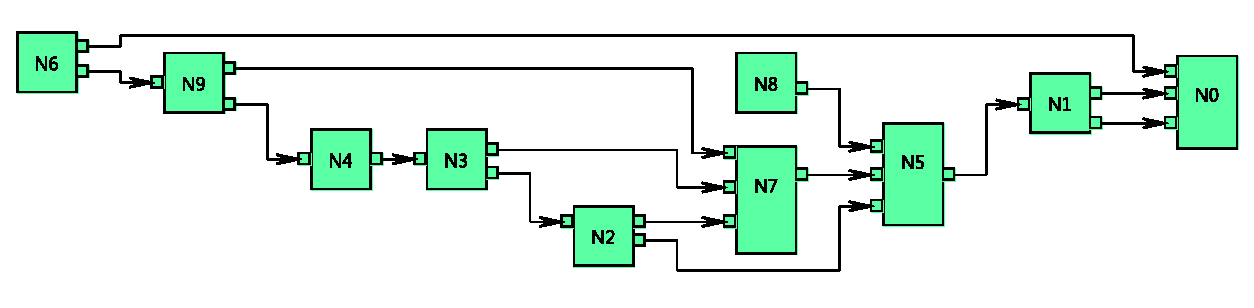
\includegraphics[width=\textwidth]{esim1.pdf}
}
\subfigure[Vaihtelua sisältävän verkon asettelu. Toimilohkoissa on 1-4 lähtöä.]{
	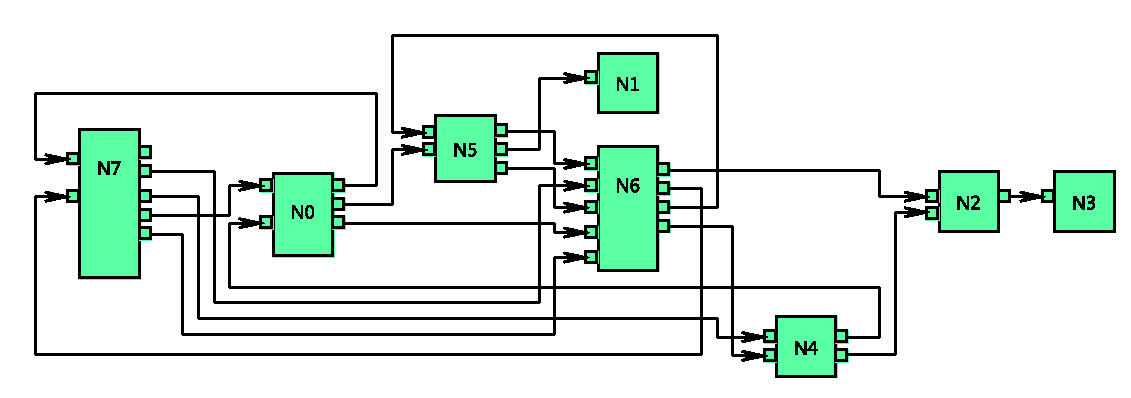
\includegraphics[width=\textwidth]{esim2.pdf}
}

\subfigure[Huomattavan monta lankaa sisältävän verkon asettelu. Jokaisesta toimilohkosta lähtee neljä lankaa.]{
	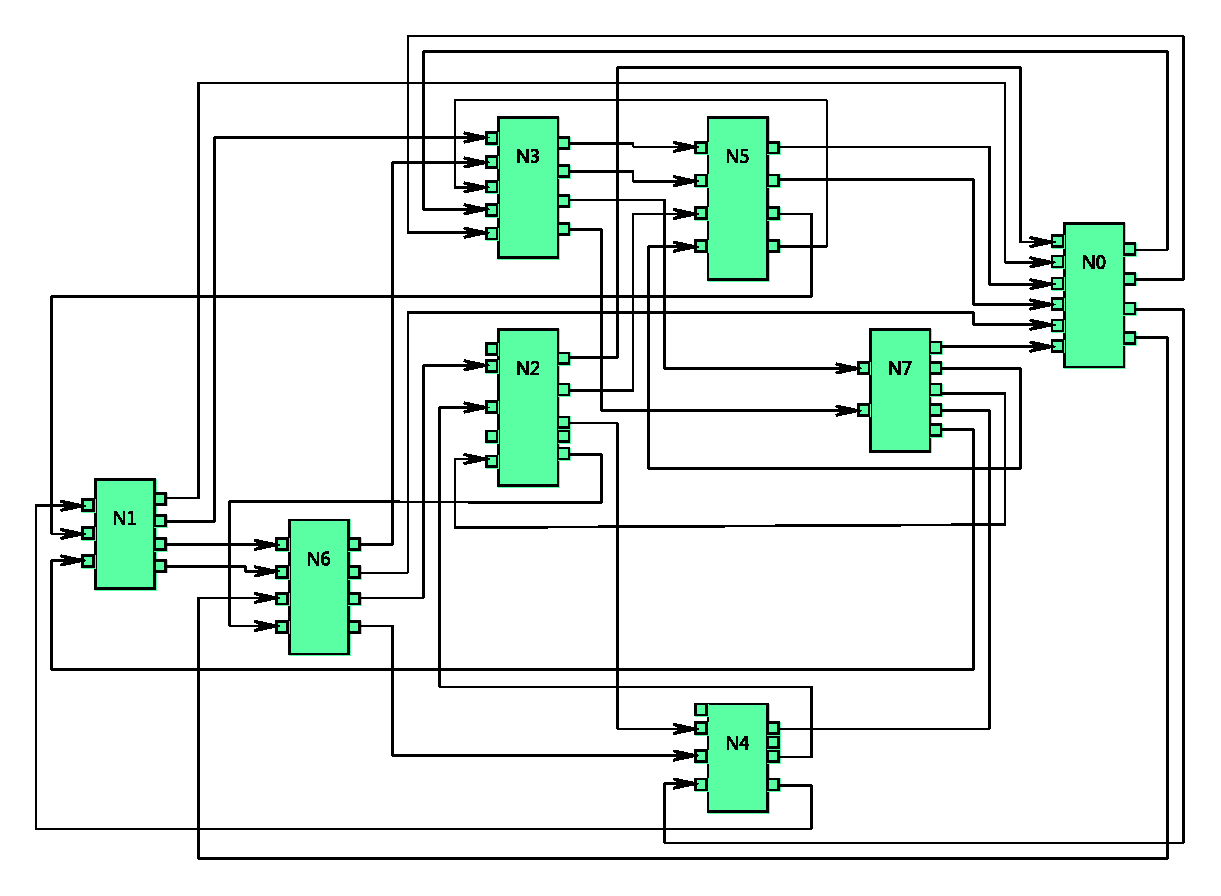
\includegraphics[width=\textwidth]{esim3.pdf}
}

\caption{Esimerkkejä algoritmin tuottamista reitityksistä. }
\end{figure}
	\clearpage

	\section{Yhteenveto}

Teollisen automaatiojärjestelmän suunnittelu- ja toteutusprosessi on monimutkainen, kallis ja pitkä.
Se käsittää suuren määrän erilaisia toimijoita, joilla voi olla 
Monet suunnitteluun liittyvistä haasteista ovat 
Siinä käytettäviä työvälineitä tehostamalla työ nopeutuu, ja voidaan saavuttaa merkittäviä säästöjä.

Työvälineiden tehostamista on akateemisissa julkaisuissa kartoitettu runsaasti.
Tutkimukset ovat kuitenkin olleet usein turhan abstrakteja ja vieraannuttavia teollisille toimijoille.
Tämä työ on pyrkinyt tarjoamaan ratkaisun, jolla suunnittelutyötä voidaan konkreettisesti tehostaa, ja joka voidaan helposti integroida olemassaoleviin järjestelmiin.

Työssä on osoitettu yhteys suunnattujen graafien ja logiikkadiagrammien välillä, sekä todettu niitten asetteluun kehitettyjen algoritmien käyttökelpoisuus teollisuuden automaatiosuunnittelussa.
Esitelty algoritmi tuottaa hyviä tuloksia, ja on muunneltavissa edelleen erilaisiin tarpeisiin.

Vaikka idea olisi hyvä ja käytännöllinen, se ei välttämättä ole kannattava.
Tästä johtuen on paljon hyviäkin ideoita, joita ei toteuteta.
Jotta yritys voi varmistaa kilpailukykynsä myös tulevaisuudessa, tulee sen arvioida jatkuvasti toteutuskelpoisten kehitysprojektien kannattavuutta, ja toteuttaa niitä harkintansa mukaan.

Automaatiojärjestelmien suunnittelu- ja ohjelmointityö on muuttunut nopeasti viime vuosikymmeninä, ja on todennäköistä että se muuttuu edelleen.


\clearpage
\addcontentsline{toc}{section}{Viitteet}

\bibliography{kandi}

\end{document}